\begin{Exercise}[title=]
  On s'interesse à un jeu de fete forraine:
  \begin{center}
    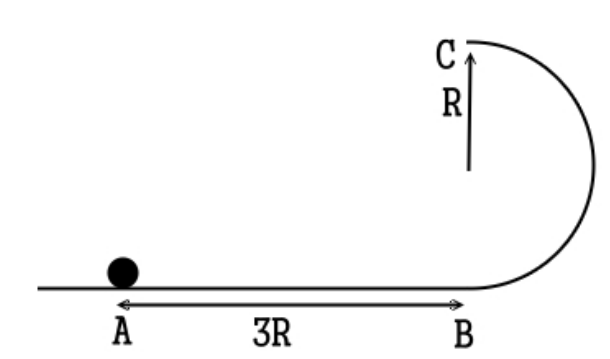
\includegraphics[width=0.4\textwidth]{fete_forraine.png}
  \end{center}
  \Question On lance un balle $M$ de masse $m$ avec une vitesse $\vec{v_0}$ à
  une distance $3R$ d'une gouttière cylindrique. La balle doit arriver en haut
  du pipe en $C$ et retomber à son point de départ en $A$ . La balle se déplace sans
  frottements.
  \Question Calculez la vitesse $v_0$ nécessaire à la balle pour atteindre le
  point $C$ . Quelle est alors sa vitesse ?
  \Question En supposant que la balle atteint le point $C$ , à quelle distance
  retombe-t-elle au sol ?
  \Question  Déterminer la vitesse pour gagner le jeu.
\end{Exercise}
\begin{Answer}
  \Question $v_B=v_A$
  \Question $v=\sqrt{2gh}$ avec une vitesse nulle en C ( toute l'énergie
  cinétique a été transformée)

  \Question chute libre $y=\frac{-gx^2}{2v_c^2}+2R$ la balle arrive en
  $x_0=\sqrt{4Rv_c^2/g}$
  \Question pour gagner le jeu il faut donc $v_c=\sqrt{\frac{9gR}{4}}$ on a donc
  $v_0=sqrt(v_c^2+2gh)$
\end{Answer}
